\documentclass{beamer}
\usepackage[T2A]{fontenc}
\usepackage[utf8]{inputenc}
\usepackage[english]{babel}
\usepackage{amssymb,amsfonts,amsmath,mathtext}
\usepackage{cite,enumerate,float,indentfirst}
\usepackage[dvips]{graphicx}
\usepackage[linesnumbered,ruled,vlined]{algorithm2e} % NEW

\setbeamertemplate{footline}[page number]

\title[\insertframenumber/\inserttotalframenumber]
{A Study of Hybrid Similarity Measures for Semantic Relation Extraction}

\author[Alexander Panchenko and Olga Morozova]
{\textbf{Alexander Panchenko and Olga Morozova}, \\ Center for Natural Language Processing (CENTAL),\\ Université catholique de Louvain, Belgium \\ {\scriptsize \url{alexander.panchenko@student.uclouvain.be} \url{olga.morozova@uclouvain.be} }}

\AtBeginSubsection[]
{
  \begin{frame}<beamer>
    \frametitle{Plan}
    \tableofcontents[currentsection,currentsubsection]
  \end{frame}
}


\mode<presentation>
{
%\usetheme{Warsaw}
\usetheme{Singapore}
\usecolortheme{orchid}%whale
\useoutertheme{smoothbars}
%\usefonttheme{serif}
}

\setbeamertemplate{navigation symbols}{%
}

\begin{document}

\begin{frame}
  \titlepage
\end{frame}

\begin{frame}
  \setcounter{tocdepth}{1}
  \frametitle{Plan}
  \tableofcontents
  \setcounter{tocdepth}{2}
	
\end{frame}

\section{Introduction}
\subsection{}


%%%%%%%%%%%%%%%%%%%%%%%%%%%%%%%%%%%%%%%%%%%%%%%%%
\begin{frame}
\frametitle{Semantic Relations}


\begin{itemize}
\item \textbf{Semantic relations} are
useful for NLP and IR applications:
\begin{itemize}
  \item Query expansion (Hsu et al., 2006)
  \item QA systems (Sun et al., 2005)	
  \item Text categorization (Tikk et al, 2003)
  \item Word Sense Disambiguation (Patwardhan et al., 2003)
\end{itemize}

\pause

\item \textbf{Semantic resources:} thesauri, ontologies, synonymy dictionaries, WordNets, \ldots

\item In the context of this work we consider following relation types: 
\begin{itemize}
\item \textbf{synonyms}: $\langle car,SYN,vehicle \rangle, \langle animal,SYN,beast \rangle$ 
\item \textbf{hypernyms} : $\langle car,HYPER,Jeep \text{ } Cherokee \rangle, \langle animal,HYPER, crocodile \rangle$
\item \textbf{co-hyponyms} (have a common hypernym):
$\langle Toyota \text{ } Land  \text{ }Cruiser,COHYPER,Jeep \text{ } Cherokee \rangle$
\end{itemize}
\end{itemize}	
\end{frame}


\begin{frame}
\frametitle{Motivation}

\begin{figure}	
	\centering
		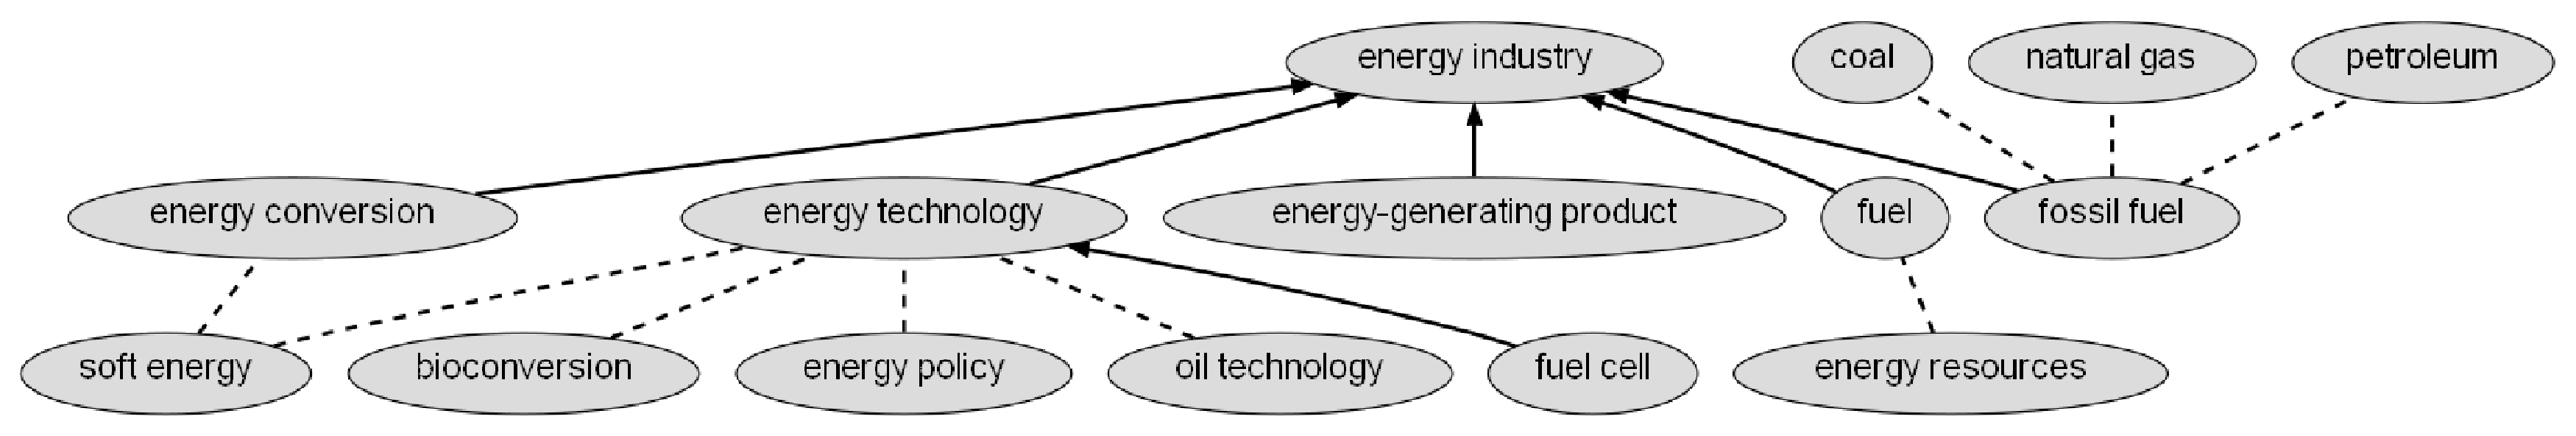
\includegraphics[width=1.0\textwidth]{figures/thesaurus2}
		\caption{Semantic relations in the EuroVoc thesaurus.}
\end{figure}

\pause
\begin{itemize}
  
\item \textbf{Manual construction of relations}:
\begin{itemize}
\item (+) Precision 
\item (--) Very expensive and time-consuming
\end{itemize}


\item \textbf{Existing relation extraction methods}:
\begin{itemize}
  \item (+) No or very little manual labor
  \item (--) Not as precise as manual construction  
  \end{itemize}

\pause

\item $\Longrightarrow$ development of \textbf{new relation extraction
methods}:
\begin{itemize}
  \item \alert{Input:} terms $C$
 \item \alert{Output:} semantic relations $\hat{R} \subset C \times C$  
\end{itemize}
\end{itemize}


\end{frame}


%%%%%%%%%%%%%%%%%%%%%%%%%%%%%%%%%%%%%%%%%%%%%%%%%%
\begin{frame}
\frametitle{The State of Art}
\begin{itemize}
\item A multitude of \textbf{complimentary measures} were proposed to extract synonyms, hypernyms,
and co-hyponyms

\item Most of them are based on \textbf{one} of the \textbf{5 key approaches}: 
\begin{enumerate}
\item distributional analysis (Lin, 1998b)
\item Web as a corpus (Cilibrasi and Vitanyi, 2007)
\item lexico-syntactic patterns (Bollegala et al., 2007)
\item semantic networks (Resnik, 1995)
\item definitions of dictionaries or encyclopedias (Zesch et al., 2008a)
\end{enumerate}

\pause


\item Some attempts were made to \textbf{combine measures} (Curran, 2002; Cederberg and Widdows, 2003; Mihalcea et al., 2006;
Agirre et al., 2009; Yang and Callan, 2009)


\item However, most studies are still \textbf{not taking into account}
all 5 existing extraction approaches.

\end{itemize}
%\textbf{Research Question}: How to combine the baseline similarity measures to improve relation extraction? 

\end{frame}


%%%%%%%%%%%%%%%%%%%%%%%%%%%%%%%%%%%%%%%%%%%%%%%%%%
\begin{frame}
\frametitle{Contributions}
\begin{itemize}
\item A systematic analysis of 
\begin{itemize}
  \item \textbf{16 baseline similarity measures} of 5 key extraction principles
  \item their combinations with \textbf{8 fusion methods} and 3 techniques for the combination set selection
\end{itemize}

\item We are first to propose \textbf{hybrid similarity measures} based on  all the 5 key extraction approaches:
\begin{enumerate}
  \item distributional analysis
  \item Web as a corpus 
  \item	lexico-syntactic patterns
  \item	semantic networks 
  \item definitions of dictionaries or encyclopedias 
\end{enumerate}

\item The best found hybrid measure combines 15 baseline measures with the Logistic Regression
 

\end{itemize}

\end{frame}


%%%%%%%%%%%%%%%%%%%%%%%%%%%%%%%%%%%%%%%%%%%%%%%%%
\section{Methodology}
\subsection{Similarity-based Relation Extraction}

\begin{frame}
\frametitle{Similarity-based Relation Extraction}

\begin{figure}
	\centering
		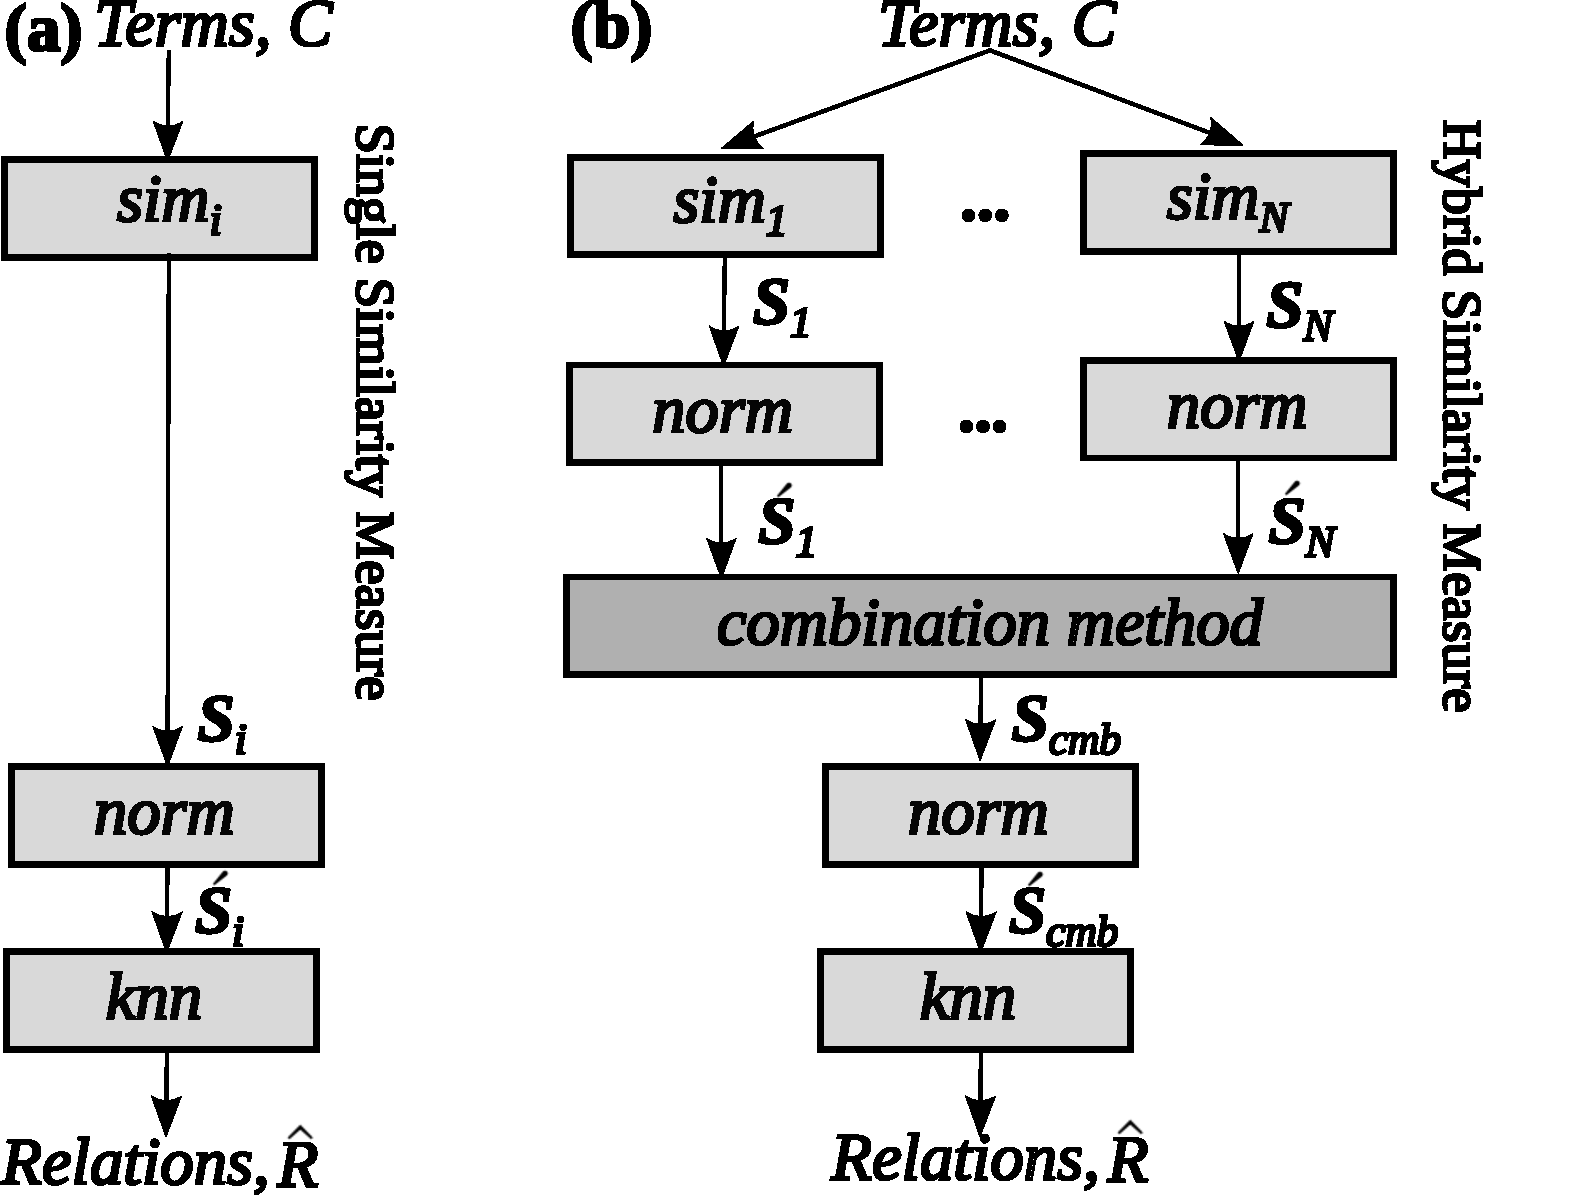
\includegraphics[width=0.40\textwidth]{figures/single-and-hybrid-2}
	\caption{Single (a) and (b) hybrid similarity-based relation extractors.}		
\end{figure}

\begin{itemize}
\item $sim_k$ -- a similarity measure $sim_k(c_i,c_j) \in [0;1], c_i,c_j \in C$
\item $\mathbf{S}_i$ -- term-term similarity matrix ($C \times C$) 

\item $knn$ -- $k$-NN thresholding:
$\hat{R}=\bigcup_{i=1}^{|C|}\left\{\left\langle c_i, c_j \right\rangle :  (c_j
\in \text{ top }k\% \text{ of } c_i) \wedge (s_{ij} > 0) \right\}.$  
\item $\mathbf{S}_{cmb}$ -- combined similarity matrix obtained with $ combination\_method(\mathbf{S}_1, \ldots,\mathbf{S}_N) $
\end{itemize}

\end{frame}

\begin{frame}
\frametitle{Single and Hybrid Similarity Measures}
\begin{itemize}
\item 16 \textbf{single} measures
	\begin{itemize}
	\item 5 measures based on a \textbf{semantic network} 
	\item 3 \textbf{web-based} measures
	\item 5 \textbf{corpus-based} measures 
	\begin{itemize}
	  \item 2 distributional
	  \item 1 lexico-syntactic patterns
	  \item 2 other co-occurence based
	\end{itemize}
	\item 3 \textbf{definition-based} measures 
\end{itemize}
\item 64 \textbf{hybrid} measures
	\begin{itemize}
	\item 8 \textbf{combination methods}
	\item 8 \textbf{measure sets} obtained with 3 measure selection techniques
	\end{itemize}
\end{itemize}

\end{frame}


\subsection{Single Similarity Measures}

%%%%%%%%%%%%%%%%%%%%%%%%%%%%%%%%%%%%%%%%%%%%%%%%%
\begin{frame}
\frametitle{Measures Based on a Semantic Network}

\begin{enumerate}
  \item Wu and Palmer (1994)
 \item Leacock and Chodorow (1998)
 \item Resnik (1995)
 \item Jiang and Conrath (1997)
 \item Lin (1998)
\end{enumerate}


 \textbf{Data:} 
 \begin{itemize}
   \item WordNet 3.0
   \item SemCor corpus
	
 \end{itemize}
 \textbf{Variables:}
 \begin{itemize}
  \item Lengths of the shortest paths between terms in the network
 \item Probability of terms derived from a corpus
 \end{itemize}
 
 \textbf{Coverage:} 155.287 English terms encoded in WordNet 3.0.
 \textbf{Complexity:} calculation of a shortest path(s) between the nodes.

\end{frame}

%%%%%%%%%%%%%%%%%%%%%%%%%%%%%%%%%%%%%%%%%%%%%%%%%
\begin{frame}
\frametitle{Web-based Measures}
	
Normalized Google Distance (NGD) (Cilibrasi and Vitanyi, 2007)

\begin{enumerate}
   \setcounter{enumi}{5}
   \item NGD-Yahoo! 
   \item NGD-Bing 
   \item NGD-Google over wikipedia.org domain     
\end{enumerate}

\textbf{Data:} number of times the terms co-occur in the documents
as indexed by an IR system.

\textbf{Variables:} 

\begin{itemize}
	\item \textbf{number of hits} returned by query $"c_i"$ 
	\item \textbf{number of hits} returned by query $"c_i \text{ AND } c_j''$
\end{itemize}

\textbf{Coverage:} huge vocabulary in dozens of languages.


\textbf{Complexity:} constraints of a search engine API.

\end{frame}

%%%%%%%%%%%%%%%%%%%%%%%%%%%%%%%%%%%%%%%%%%%%%%%%%
\begin{frame}
\frametitle{Corpus-based Measures}

\begin{enumerate}
   \setcounter{enumi}{8}
	\item Bag-of-word Distributional Analysis (BDA) (Sahlgren, 2006) 
	\item Syntactic Distributional Analysis (SDA) (Curran, 2003) 
\end{enumerate}

\textbf{Data:} WaCkypedia (800M tokens) and PukWaC (2000M tokens) corpora (Baroni et al., 2009) 
 
\textbf{Variables:} 
\begin{itemize}
  \item feature vector based on the \textbf{context window}
  \item feature vector based on the \textbf{syntactic context} 
\end{itemize}

\textbf{Coverage:} word should occur in the corpora.

\textbf{Complexity:} O(BDA) << O(SDA) because of dependency parsing
	
\end{frame}

%%%%%%%%%%%%%%%%%%%%%%%%%%%%%%%%%%%%%%%%%%%%%%%%%
\begin{frame}
\frametitle{Corpus-based Measures }

\begin{enumerate}
  \setcounter{enumi}{10}
  \item A measure based on \textbf{lexico-syntactic patterns} (PatternWiki) 
\end{enumerate}	
 
\textbf{Data}: WaCkypedia corpus (800M tokens) 

\textbf{Method:}
\begin{itemize}
	\item 10 patterns for hypernymy extraction: 6 Hearst (1992) patterns + 4 other patterns
	\item \texttt{such diverse \{[occupations]\} as
  \{[doctors]\}, \{[engineers]\} and \{[scientists]\}[PATTERN=1]}
  
  \item Semantic similarity $s_{ij}$ between terms $c_i, c_j \in C$ is a function of 
 the number of term co-occurences in the same concordance $n_{ij}$:
  
   $$
   sim(c_i,c_j) = s_{ij} = \frac{n_{ij}}{max_{ij}(n_{ij})}.
   $$
\end{itemize}
 
 \end{frame}
 
 \begin{frame}
\frametitle{Corpus-based Measures}
	
 \begin{figure}
        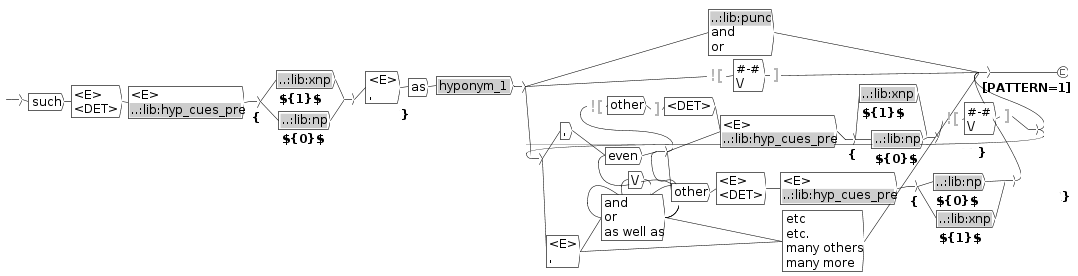
\includegraphics[width=1.0\textwidth]{figures/hypernym_1}
        \caption{A UNITEX graph implementing the first extraction pattern.}
        \label{fig:prcomb}
\end{figure}

\textbf{Coverage:} Target terms $c_i, c_j$ should co-occur in a sentence.
\textbf{Complexity:} Application of a cascade of FST to a text.
	
\end{frame}

\begin{frame}
\frametitle{Corpus-based Measures }

\begin{enumerate}
   \setcounter{enumi}{11}
	\item \textbf{Latent Semantic Analysis (LSA)} on TASA corpus (Landauer and Dumais, 1997)
	\item \textbf{NGD} on Factiva corpus (Veksler et al., 2008)
\end{enumerate}
	
\end{frame}

%%%%%%%%%%%%%%%%%%%%%%%%%%%%%%%%%%%%%%%%%%%%%%%%%
\begin{frame}
\frametitle{Definition-based Measures}

\begin{enumerate}
  \setcounter{enumi}{13}
  \item \textbf{Extended Lesk}  (Banerjee and Pedersen, 2003)
  \item \textbf{GlossVectors} (Patwardhan and Pedersen, 2006)
\end{enumerate}


\textbf{Data:} WordNet glosses.
	
\textbf{Variables:}
\begin{itemize}
		\item bag-of-words vector of a term $c_i$ derived from the glosses
		\item relation  between words $(c_i,c_j)$ in the network 
\end{itemize}

\textbf{Coverage:} 117.659 glosses encoded in WordNet 3.0

\textbf{Complexity:} Calculation of a similarity in a vector space.

\end{frame}


%%%%%%%%%%%%%%%%%%%%%%%%%%%%%%%%%%%%%%%%%%%%%%%%%
\begin{frame}
\frametitle{Definition-based Measures}

\begin{enumerate}
 \setcounter{enumi}{15} 
\item \textbf{WktWiki} -- BDA on definitions of Wiktionary and Wikipedia~\footnote{The method stems from the work of Zesch et al. (2008)}

\end{enumerate}

\textbf{Data}: Wikipedia abstracts, Wiktionary.

\textbf{Method:}
\begin{itemize}
  \item Definition = abstract of Wikipedia article with title $"c_i"$ + 
   glosses, examples, quotations, related words, categories from Wiktionary  for $c_i$
   \item Represent a definition as a bag-of-words vector
   \item Calculate similarities with cosine
   \item Update similarities according to relations in the Wiktionary.
  
\end{itemize}
   \textbf{Coverage:} Wiktionary: 536.594 glosses, Wikipedia: 3.8M articles
   
   \textbf{Complexity:} Cosine calculation in a bag-of-words space. 
  
\end{frame}


\subsection{Hybrid Similarity Measures}

%%%%%%%%%%%%%%%%%%%%%%%%%%%%%%%%%%%%%%%%%%%%%%%%%
\begin{frame}
\frametitle{Combination Methods}
\begin{itemize}
\item A \textbf{goal of a combination method} is to produce ``better'' similarity scores than the
scores of single measures.

\item A \textbf{combination method} takes as an input   
$\{\mathbf{S}_1,\ldots,\mathbf{S}_K\}$ produced by $K$ single measures and
outputs  $\mathbf{S}_{cmb}$.

\item $s_{ij}^k \in \mathbf{S}_k$ is a \textbf{pairwise similarity score} of terms $c_i$ and $c_j$ produced by $k$-th measure.

\item We tested \textbf{8  combination methods}.

\end{itemize}
\end{frame}

\begin{frame}
\frametitle{Combination Methods}

\begin{enumerate}
  
\item \textbf{Mean}. A mean of $K$ pairwise similarity scores:

$$\mathbf{S}_{cmb} = \frac{1}{K} \sum_{k=1}^K \mathbf{S}_k \Leftrightarrow 
s_{ij}^{cmb}= \frac{1}{K}\sum_{k=1,K} s_{ij}^k.$$

\item \textbf{Mean-Nnz}. A mean of scores having non-zero value:
 $$s_{ij}^{cmb}= \frac{1}{|k:s_{ij}^k
>0,k=1,K|}\sum_{k=1,K} s_{ij}^k.$$

\item \textbf{Mean-Zscore}. A mean of scores
transformed into Z-scores:
$$\mathbf{S}_{cmb} = \frac{1}{K} \sum_{k=1}^K \frac{\mathbf{S}_k -
\mu_k}{\sigma_k},$$ where $\mu_k$ and $\sigma_k$ are a mean and a standard deviation of the scores of the $k$-th measure ($\mathbf{S}_k$).

\end{enumerate}
\end{frame}



\begin{frame}
\frametitle{Combination Methods}

\begin{enumerate}
  \setcounter{enumi}{3}
\item \textbf{Median}. A median of $K$ pairwise similarities:
$$s_{ij}^{cmb}= median(s_{ij}^1,\ldots,s_{ij}^K). $$

\item \textbf{Max}. A maximum of $K$ pairwise similarities:
$$s_{ij}^{cmb}= max(s_{ij}^1,\ldots,s_{ij}^K).$$

\item \textbf{RankFusion}. A mean of scores converted to ranks:
 $$s_{ij}^{cmb}= \frac{1}{K}\sum_{k=1,K}
r_{ij}^k,$$
where  $r^k_{ij}$ is the rank corresponding to the similarity score $s^k_{ij}$.
\end{enumerate}

\end{frame}



\begin{frame}
\frametitle{Combination Methods}

\begin{enumerate}
  \setcounter{enumi}{6}
  \item \textbf{RelationFusion}. Unions the best relations found by each measure separately. A relation  extracted independently by several method has more weight. 

\begin{algorithm}[H]
\SetLine
\KwIn{Similarity matrices of $N$ single measures $\{\mathbf{S}_1,\ldots,\mathbf{S}_N\}$, number of nearest neighbors $K$}
\KwOut{ Combined similarity matrix $\mathbf{S}_{cmb}$  }

\For{i=1,N}{
	$R_i = knn(\mathbf{S}_i, k)$ \;
 	$\mathbf{R}_i = relation\_matrix(R_i)$
 }
$\mathbf{S}_{cmb} = \frac{1}{N} \sum_{i=1}^N \mathbf{R}_i$ \;
\Return $\mathbf{S}_{cmb}$ \;
\label{rfusion}
\end{algorithm}
$$
r^k_{ij} \in \mathbf{R}_k, r_{ij}^k = \left\{ 
  \begin{array}{l l}
    1 & \quad \text{if relation } \langle c_i, c_j \rangle \in R_k \\
    0 & \quad \text{else}\\
  \end{array} \right.
$$

\end{enumerate}

\end{frame}


\begin{frame}
\frametitle{Combination Methods}

\begin{enumerate}
  \setcounter{enumi}{7}
\item \textbf{Logit}. 
 A supervised combination of similarity measures 

\begin{itemize}
  \item  Training a \textbf{binary classifier} (a Logistic Regression) on a set of manually constructed
semantic relations $R$ (BLESS or SN)

\item \textbf{Positive training examples} are “meaningful” relations (synonyms,
hyponyms, co-hyponyms, associations)
\item \textbf{Negative training examples} are pairs of semantically unrelated words (generated randomly and verified manually).


  \item A relation $\langle c_i,t, c_j \rangle \in R$ is represented with an $N$-dimensional \textbf{vector of pairwise similarities}: $\mathbf{x}_{ij} = (s_{ij}^1,\ldots,s_{ij}^N)$. 

\item Category $y_{ij}$:
$$
y_{ij} = \left\{ 
  \begin{array}{l l}
    0 & \quad  \text{ if } \langle c_i,t, c_j \rangle \text{ is a random relation} 
    \\
    1 & \quad  \text{ otherwise }\\
  \end{array} \right
  .
$$

\item \textbf{Using the model} $(w_1,\ldots,w_K)$ to combine measures: 
$$s^{cmb}_{ij} = \frac{1}{1 + e^{-z}}, z = w_0 + \sum_{k=1}^K w_k s^k_{ij} , $$

\end{itemize}
\end{enumerate}

\end{frame}

%%%%%%%%%%%%%%%%%%%%%%%%%%%%%%%%%%%%%%%%%%%%%%%%%
\begin{frame}
\frametitle{Combination Sets}

\begin{block}{A problem}
 Number of ways to choose which of 16 single measures to combine with one combination method:

$$\sum_{m=2}^{16}C_{16}^m=\sum_{m=2}^{16}\frac{16!}{m!(16-m)!}=65.535$$
 
\end{block}

\begin{itemize}
 
\item \textbf{Expert choice of measures} -- 5, 9 and 15 measures
\item \textbf{Forward Stepwise Procedure} -- 7, 8a, 8b, 10 measures 
\item \textbf{Analysis of a Logistic Regression} weights trained on 16 measures
 -- 12 measures

\pause

\item The \alert{best single predictors} of relations: C-BDA, C-SDA, C-LSA-Tasa, D-WktWiki, D-GlossVectors,  D-ExtendedLesk.

%\begin{itemize}
 %\item \textbf{5} % = WN-Resnik, BDA-3-5000, SDA-21-100000,  Def-WktWiki-1000
 %\item \textbf{9} %= \textbf{Group4} + WN-WuPalmer, LSA-Tasa, Def-GlossVec., and Def-Ext.Les
 %\item \textbf{15} %= \textbf{Group8} + WN-LeacockChodorow, WN-Lin, WN-JiangConrath, NGD-Factiva, NGD-Yahoo, and NGD-GoogleWiki.
%\end{itemize}

\end{itemize}
\end{frame}
  

%%%%%%%%%%%%%%%%%%%%%%%%%%%%%%%%%%%%%%%%%%%%%%%%%
\section{Evaluation}
\subsection{}

%%%%%%%%%%%%%%%%%%%%%%%%%%%%%%%%%%%%%%%%%%%%%%%%%
\begin{frame}
\frametitle{Human Judgement Datasets}

\begin{table}[h]\footnotesize
\begin{tabular}{ |c|c|c|c|c|c| }
\hline
  term, $c_i$ & term, $c_j$ & judgement, $\mathbf{s}$  & sim, $\mathbf{s}$  & judgement, $\mathbf{r}$ & sim, $\hat{\mathbf{r}}$  \\ \hline \hline
tiger & cat & 7.35 & 0.85 & 1 & 3 \\
book & paper & 7.46 &  0.95 & 2 & 2 \\
computer & keyboard & 7.62 &  0.81 & 3 & 1 \\
... & ... & ... & ...   & \ldots & \ldots \\
possibility & girl & 1.94 & 0.25 & 64 & 65 \\
sugar & approach & 0.88 & 0.05 & 65 & 23 \\ \hline
\end{tabular}
\end{table}


\textbf{Data:}

\begin{itemize}
	\item WordSim353 -- 353 term pairs (Finkelstein, 2002)  
	\item MC -- 30 term pairs  (Miller & Charles, 1991)
	\item RG -- 65 term pairs (Rubenstein & Goodenough, 1965)  
\end{itemize}

\textbf{Criteria:}
\begin{itemize}
\item Pearson correlation:  $\rho = \frac{cov(\mathbf{s},\hat{\mathbf{s}})}{\sigma(\mathbf{s}) \sigma(\hat{\mathbf{s}})}$

 \item Spearman's correlation: $r = \frac{cov(\mathbf{r},\hat{\mathbf{r}})}{\sigma(\mathbf{r}) \sigma(\hat{\mathbf{r}})}$
 
 \end{itemize}
 
\end{frame}


%%%%%%%%%%%%%%%%%%%%%%%%%%%%%%%%%%%%%%%%%%%%%%%%%
\begin{frame}
\frametitle{Semantic Relation Datasets: Data}

{ \scriptsize

\begin{table}[h]\footnotesize
\begin{tabular}{ |c|l|l| }
\hline
term, $c_i$ & term, $c_j$ & relation type, $t$  \\ \hline \hline
judge & adjudicate & syn \\
judge & arbitrate & syn \\
%judge & asessor & syn \\
judge & chancellor & syn \\
%judge & gendarmerie & syn \\
judge & sheriff & syn \\
... & ... & ...   \\
judge & pc & random \\ 
judge & fare & random \\
judge & lemon & random \\ \hline
\end{tabular}
\end {table}

}

\begin{itemize}
  \item \textbf{BLESS} (Baroni and Lenci, 2011)
  \begin{itemize}
    \item 26554 relations
    \item hyperonyms, co-hypernyms, meronyms, associations, attributes, random relations
    \end{itemize}  
  \item \textbf{SN} (Semantic Neighbors)
  \begin{itemize}
    \item 14682  relations\
    \item synonyms, random relations
    \end{itemize}
    
    \item $|R_{random}|/|R_{rest}| \approx 0.5$
     
\end{itemize}

\end{frame}

%%%%%%%%%%%%%%%%%%%%%%%%%%%%%%%%%%%%%%%%%%%%%%%%%
\begin{frame}
\frametitle{Semantic Relation Datasets: Criteria}

\begin{itemize}
  
  \item Based on the number of correctly extracted (ranked) relations.
  

\item $R$ -- all not random semantic relations 

\item $\hat{R}(k)$ --  extracted relations if the number of nearest neighbors is $k$

\begin{block}{Criteria}

	
	\begin{itemize}
		\item Precision: $P(k)=$$\frac{|R \cap \hat{R}(k)|}{|\hat{R}(k)|}$,
		\item Recall: $R(k)=$$\frac{|R \cap \hat{R}(k)|}{|R|}$,
		\item F1-measure: $F(k)= 2 \cdot \frac{P(k) \cdot R(k)}{P(k) + R(k)}$,
		\item MAP $M(k) = \frac{1}{k}\sum^{k}_{i=1}P(i)$.
	\end{itemize}	
	\end{block}

\item We use $P(10)$, $P(20)$, $P(50)$, $R(50),M(20)$, $M(50)$.
	

\end{itemize}
	
	
\end{frame}


%%%%%%%%%%%%%%%%%%%%%%%%%%%%%%%%%%%%%%%%%%%%%%%%%
\begin{frame}
\frametitle{Semantic Relation Datasets: Example}

\begin{itemize}
	\item Precision $P(50\%)= \frac{1}{7} \approx 0.86 $
\end{itemize}


\begin{table}[h]\footnotesize
\begin{tabular}{ |l|l|l|l| }
\hline
 term, $c_i$ &  term, $c_j$ & relation type & \bf $s_{ij}$ \\ \hline \hline

aficionado & enthusiast & syn & 0.07197 \\
aficionado & fan & syn & 0.05195 \\
aficionado & admirer & syn & 0.01964 \\
aficionado & addict & syn & 0.01326 \\
aficionado & devotee & syn & 0.01163 \\
aficionado & foundling & random & 0.00777 \\
aficionado & fanatic & syn & 0.00414 \\ \hline
aficionado & adherent & syn & 0.00353 \\
aficionado & capital & random & 0.00232 \\
aficionado & statute & random & 0.00029 \\
aficionado & blot & random & 0.00025 \\
aficionado & meddler & random & 0.00005 \\
aficionado & enlargement & random &	0.00003 \\
aficionado & bawdyhouse & random & 	0.00000 \\ 
\hline
\end{tabular}
\end {table}

\end{frame}

\section{Results}
\subsection{}

%%%%%%%%%%%%%%%%%%%%%%%%%%%%%%%%%%%%%%%%%%%%%%%%%

\begin{frame}
\frametitle{Single Similarity Measures}
	\begin{figure}
	\centering
		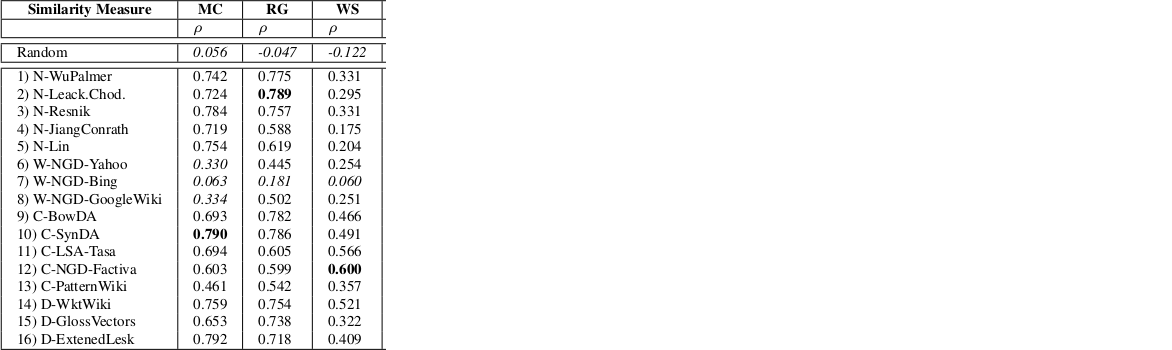
\includegraphics[width=1.0\textwidth]{figures/table-hybrid-single-hg}
		
		\caption{ Performance of \textbf{16 single similarity measures} on \textbf{human judgement datasets} (MC, RG,
WordSim353). The best scores in a group are in
bold. 
}
\end{figure}
	
\end{frame}


\begin{frame}
\frametitle{Single Similarity Measures}
	\begin{figure}
	\centering
		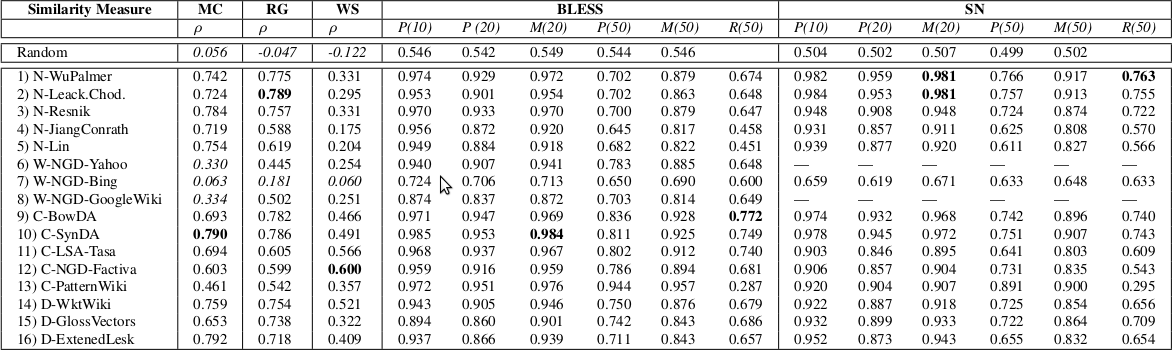
\includegraphics[width=1.0\textwidth]{figures/table-hybrid-single}
		
		\caption{ Performance of \textbf{16 single similarity measures} on human judgement datasets (MC, RG,
WordSim353) and semantic relation datasets (BLESS and SN). The best scores in a group are in
bold. 
}
\end{figure}
	
\end{frame}

%%%%%%%%%%%%%%%%%%%%%%%%%%%%%%%%%%%%%%%%%%%%%%%%%
\begin{frame}
\frametitle{Hybrid Similarity Measures}

	\begin{figure}
	\centering
		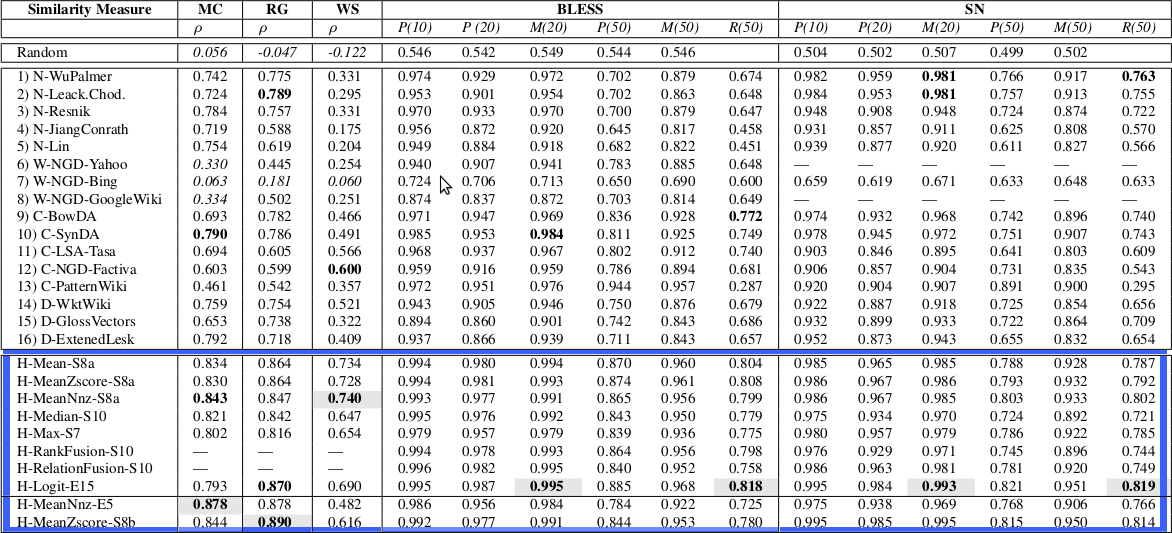
\includegraphics[width=1.0\textwidth]{figures/table-hybrid-hybrid}
		
		\caption{ Performance of \textbf{16 single and 8 hybrid similarity measures} on human judgements datasets (MC, RG,
WordSim353) and semantic relation datasets (BLESS and SN). The best scores in a group (single/hybrid) are in
bold; the very best scores are in grey. }
\end{figure}
	
	
\end{frame}

%%%%%%%%%%%%%%%%%%%%%%%%%%%%%%%%%%%%%%%%%%%%%%%%%
\begin{frame}
 \frametitle{Hybrid Similarity Measures}
	\begin{figure}
	\centering
		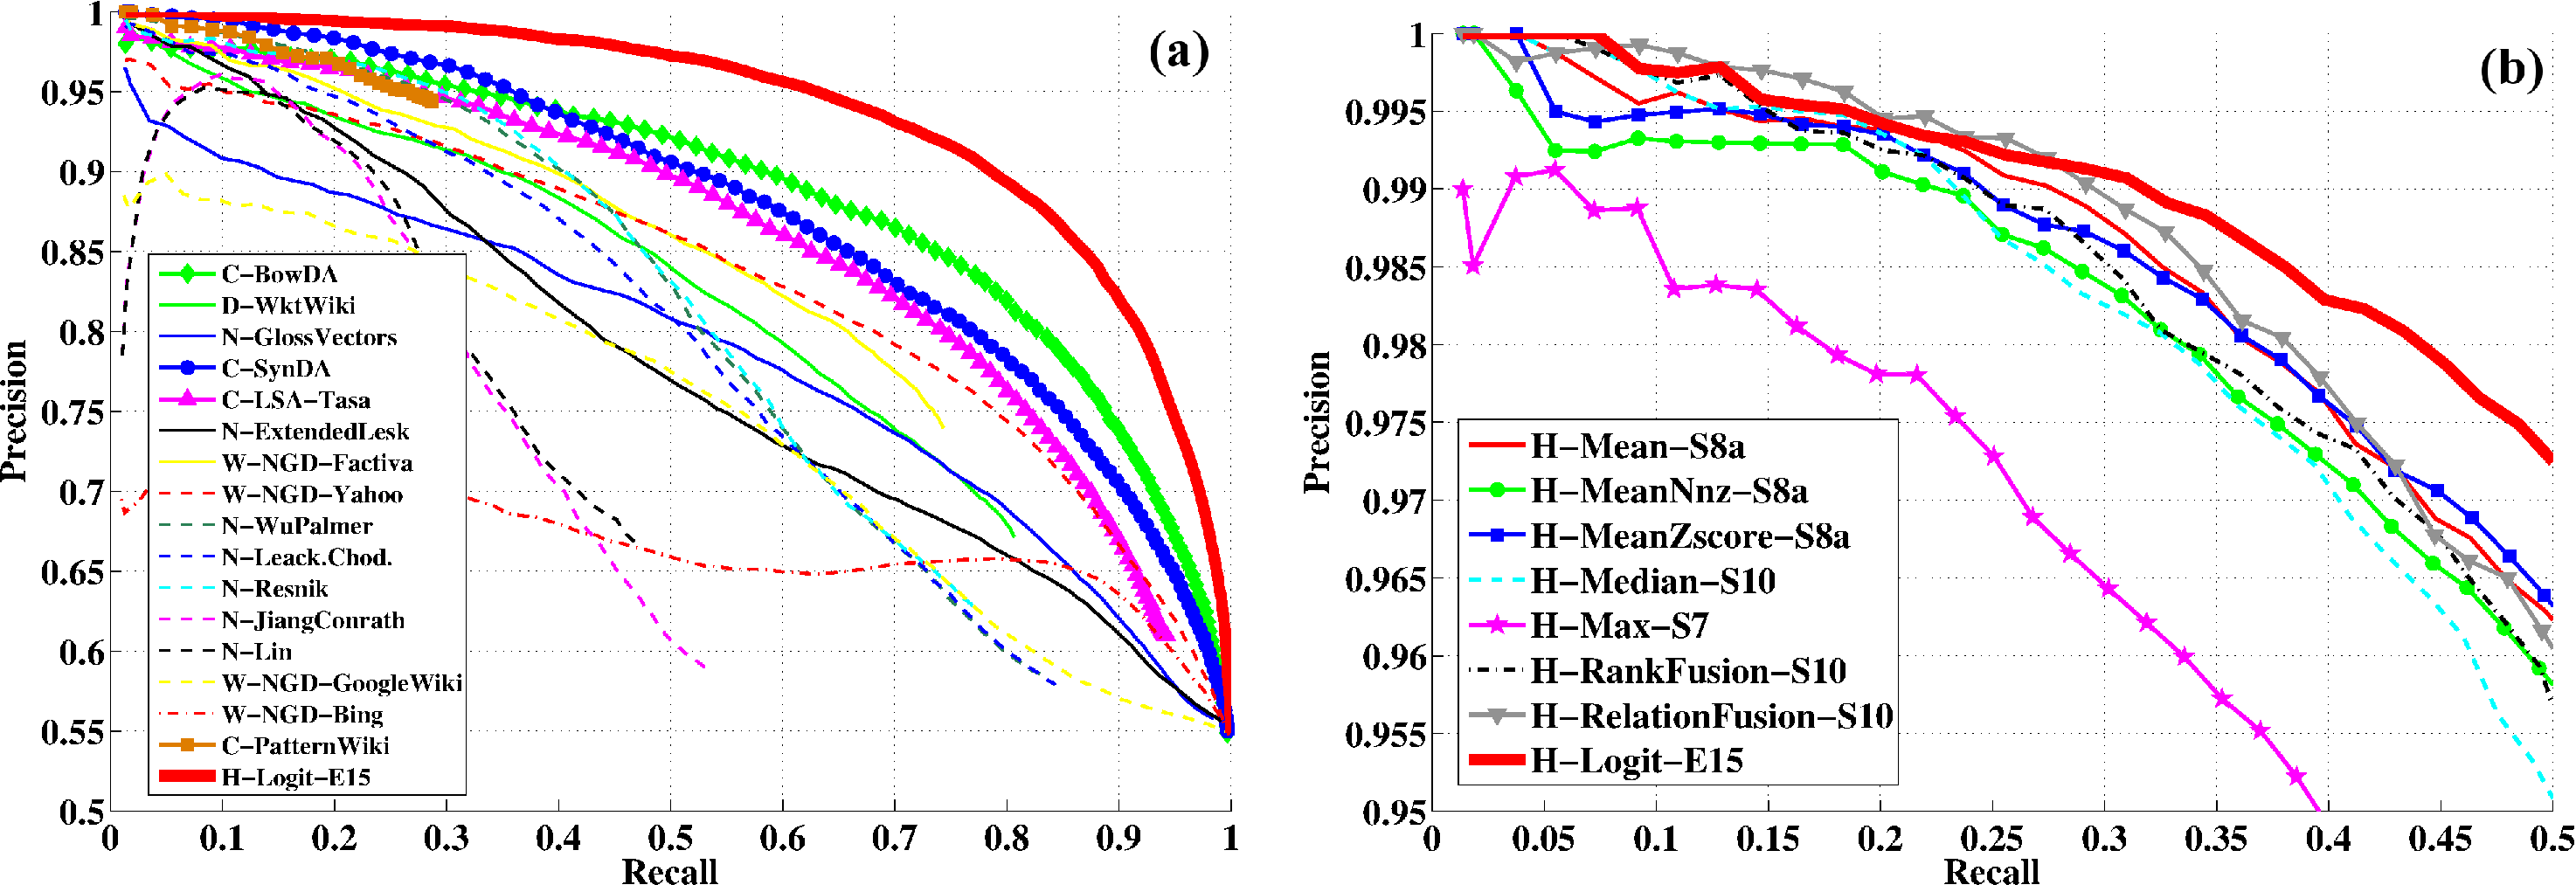
\includegraphics[width=1.0\textwidth]{figures/pr}
		\caption{Precision-Recall graphs calculated on the BLESS dataset of (a) 16 single measures and the best hybrid
measure H-Logit-E15; (b) 8 hybrid measures.}
\end{figure}
	
\end{frame}

%%%%%%%%%%%%%%%%%%%%%%%%%%%%%%%%%%%%%%%%%%%%%%%%%
\section{Conclusion}
\subsection{}

%%%%%%%%%%%%%%%%%%%%%%%%%%%%%%%%%%%%%%%%%%%%%%%%%
\begin{frame}
\frametitle{Conclusion:}

\begin{itemize}
  
%\item We designed and studied several
%hybrid similarity measures in the context of semantic relation extraction.

\item We have undertaken \textbf{a study} of 16 baseline measures, 8
combination methods, and 3 measure selection techniques.

\item The \textbf{proposed hybrid measures}:

\begin{itemize}
  \item use all 5 main types of baseline measures;
  \item outperform the single measures on all datasets.
\end{itemize}  

  
\item The \textbf{best results} were provided by
\begin{itemize}
  \item  a combination of 15  corpus-, web-, network-, and definition-based measures
\item with Logistic Regression 
\item $\rho= 0.870$, $P(20)=0.987$, $R(50)=0.814$.
\end{itemize}

\pause

\item We are going to apply the
developed methods to \textbf{query expansion} and \textbf{text classification}.
 
\end{itemize}

\end{frame}

\begin{frame}
\frametitle{}

\Huge \bf Thank you! Questions?
\end{frame}
\end{document}